%%% 
%% Copyright 2007, 2008, 2009 Elsevier Ltd
%% 
%% This file is part of the 'Elsarticle Bundle'.
%% ---------------------------------------------
%% 
%% It may be distributed under the conditions of the LaTeX Project Public
%% License, either version 1.2 of this license or (at your option) any
%% later version.  The latest version of this license is in
%c%    http://www.latex-project.org/lppl.txt
%% and version 1.2 or later is part of all distributions of LaTeX
%% version 1999/12/01 or later.
%% 
%% The list of all files belonging to the 'Elsarticle Bundle' is
%% given in the file `manifest.txt'.
%% 
%% Template article for Elsevier's document class `elsarticle'
%% with numbered style bibliographic references
%% SP 2008/03/01

%% \documentclass[preprint,review,11pt]{elsarticle}
\documentclass[final,times]{elsarticle}

%% Use the option review to obtain double line spacing
%% \documentclass[authoryear,preprint,review,12pt]{elsarticle}

%% Use the options 1p,twocolumn; 3p; 3p,twocolumn; 5p; or 5p,twocolumn
%% for a journal layout:
%\documentclass[final,1p,times]{elsarticle}
%% \documentclass[final,1p,times,twocolumn]{elsarticle}
%% \documentclass[final,3p,times]{elsarticle}
%% \documentclass[final,3p,times,twocolumn]{elsarticle}
%% \documentclass[final,5p,times]{elsarticle}
%% \documentclass[final,5p,times,twocolumn]{elsarticle}

%% For including figures, graphicx.sty has been loaded in
%% elsarticle.cls. If you prefer to use the old commands
%% please give \usepackage{epsfig}

%% The amssymb package provides various useful mathematical symbols
\usepackage{amssymb}
%% The amsthm package provides extended theorem environments
%% \usepackage{amsthm}

%% The lineno packages adds line numbers. Start line numbering with
%% \begin{linenumbers}, end it with \end{linenumbers}. Or switch it on
%% for the whole article with \linenumbers.
 \usepackage{lineno}

\usepackage{amsmath,hyperref}
\usepackage{mathrsfs}
\usepackage{bbm}
\usepackage{mathtools}
\usepackage[margin=1in]{geometry}
\usepackage{multirow}
\usepackage{subfig}
\biboptions{numbers,sort&compress}


\usepackage{algorithm}
\usepackage{algorithmic}
\usepackage{booktabs}
\usepackage[table]{xcolor}
    \definecolor{gray}{gray}{0.85}



\renewcommand{\figurename}{Fig.}
\renewcommand*{\figureautorefname}{Fig.}
\renewcommand*{\subsectionautorefname}{Sec.}
\renewcommand*{\sectionautorefname}{Sec.}
\usepackage{subfig}
\newcommand{\subfigureautorefname}{\figureautorefname}

% equation numbering (section#. equation#)
\numberwithin{equation}{section}



%% define macro
\newcommand{\pStokeslet}{\mathbb{G}}
\newcommand{\fStokeslet}{\mathbb{G}}
\newcommand{\rStokeslet}{\mathbb{G}^{(r)}}
\newcommand{\wStokeslet}{\mathbb{G}^{(w)}}
\newcommand{\B}[1]{\mathbf{#1}}
\newcommand{\V}[1]{\boldsymbol{#1}}
\newcommand{\op}[1]{\boldsymbol{\mathcal{#1}}}
\DeclareMathOperator*{\argmax}{arg\,max}
\DeclareMathOperator*{\argmin}{arg\,min}
\newcommand{\D}[1]{\dot{#1}}
\newcommand{\T}[1]{\tilde{#1}}
\newcommand{\WT}[1]{\widetilde{#1}}


\newcommand{\diff}{\mathrm{d}}
\newcommand{\myhat}[2]{\hat{#1}_{#2}}
\renewcommand*\arraystretch{1.5}
\renewcommand{\div}[1]{\nabla_{#1} \cdot}
\newcommand{\ggrad}{\nabla^2}
\newcommand{\lapl}[1]{\Delta_{#1}}
\newcommand{\grad}[1]{\nabla_{#1}}
\newcommand{\curl}{\nabla \times}
\newcommand{\Tr}{\mathrm{Tr}}

\newcommand{\dlapl}[2]{\Delta^{#1}_{#2}}
\newcommand{\dgrad}[2]{\nabla^{#1}_{#2}}
\newcommand{\ddiv}[2]{\nabla^{#1}_{#2} \cdot}


\newcommand{\Mwave}{\mbf{M}^{(w)}}
\newcommand{\Mreal}{\mbf{M}^{(r)}}
\newcommand{\sqrtM}{\mbf{M}^{1/2}}
\newcommand{\sqrtMwave}{\left(\mbf{M}^{(w)}\right)^{1/2}}
\newcommand{\sqrtMreal}{\left(\mbf{M}^{(r)}\right)^{1/2}}

\newcommand{\xir}{\xi^2 r^2}
\newcommand{\kxi}{k^2/4\xi^2}

\newcommand{\kbt}{k_BT}
\newcommand{\rcutoff}{r_c}
\newcommand{\rAlpert}{r_{\text{Alpert}}}
\newcommand{\Nbox}{N_{\text{box}}}
\newcommand{\tolEwald}{\epsilon_{\text{Ewald}}}
\newcommand{\tolIter}{\epsilon_{\text{tol}}}

% revision macro
\usepackage{color}
\PassOptionsToPackage{normalem}{ulem}
\usepackage{ulem}
%\newcommand{\redadd}[1]{#1}
\newcommand{\redadd}[1]{{\color{red}#1}}
\newcommand{\reddelete}[1]{{\color{red}\sout{#1}}}
\newcommand{\blueadd}[1]{{\color{blue}#1}}
\newcommand{\bluedelete}[1]{{\color{blue}\sout{#1}}}
\newcommand{\Donev}[1]{{{\bf \color{red}[#1]}}}
\definecolor{mygreen}{rgb}{0,.6,0}
\newcommand{\greenadd}[1]{{\color{mygreen}#1}}
\newcommand{\eric}[1]{\textcolor{blue}{\textit{#1}}}
\allowdisplaybreaks



\usepackage[nameinlink,noabbrev]{cleveref}
\crefname{equation}{eq.}{eqs.} % force abbreviated forms for equation "names"
\Crefname{equation}{Eq.}{Eqs.}
\crefname{figure}{fig.}{fiqs.}
\Crefname{figure}{Fig.}{Figs.}
\crefname{table}{tab.}{tabs.}
\Crefname{table}{Tab.}{Tabs.}


\def\appendixname{}


\newtheorem{thm}{Lemma}[section] 
\newtheorem{lem}[thm]{Lemma} 
\newdefinition{rmk}{Remark}[section]
\newproof{pf}{Proof}
\newproof{pot}{Proof of Theorem \ref{thm2}}
\newtheorem{type}{Type}






% \usepackage[inline]{showlabels}


% \journal{J. Comput. Phys.}

\begin{document}

\begin{frontmatter}

%% Title, authors and addresses

%% use the tnoteref command within \title for footnotes;
%% use the tnotetext command for theassociated footnote;
%% use the fnref command within \author or \address for footnotes;
%% use the fntext command for theassociated footnote;
%% use the corref command within \author for corresponding author footnotes;
%% use the cortext command for theassociated footnote;
%% use the ead command for the email address,
%% and the form \ead[url] for the home page:
%% \title{Title\tnoteref{label1}}
%% \tnotetext[label1]{}
%% \author{Name\corref{cor1}\fnref{label2}}
%% \ead{email address}
%% \ead[url]{home page}
%% \fntext[label2]{}
%% \cortext[cor1]{}
%% \address{Address\fnref{label3}}
%% \fntext[label3]{}

\title{Phase-Field Model for Directional Solidification in Additive Manufacturing Testbed Problems}
\author[oden]{Yuanxun Bao}
\ead{yxbao@utexas.edu}

\author[utme]{Yigong Qin}
\ead{ygqin@utexas.edu}


\author[oden]{George Biros}
\ead{biros@oden.utexas.edu}

\address[oden]{Oden Institute for Computational Engineering and Sciences, The University of Texas at Austin}
\address[utme]{Department of Mechanical Engineering, The University of Texas at Austin}


% \cortext[cor1]{Corresponding author}


%% use optional labels to link authors explicitly to addresses:
%% \author[label1,label2]{}
%% \address[label1]{}
%% \address[label2]{}

%%\author{}
%%\address{}

\begin{abstract}
In this report we present the phase-field model for directional solidification \cite{Echebarria2004,Tourret2015}, its discretization and implementation, and numerical results for several benchmark problems. 
\end{abstract}

% \begin{keyword}
%% keywords here, in the form: keyword \sep keyword

%% PACS codes here, in the form: \PACS code \sep code

%% MSC codes here, in the form: \MSC code \sep code
%% or \MSC[2008] code \sep code (2000 is the default)

% \end{keyword}

\end{frontmatter}


% \linenumber
\section{Phase-field model for directional solidification}

\subsection{Phase-field equations}
We consider the phase-field model for directional solidification of dilute binary alloys proposed by Echebarria et al. \citep{Echebarria2004} with frozen temperature approximation:
\begin{align}
    & T(z,t) = T_0 + G(z-Rt),
\end{align}
where $T_0$ is a reference temperature at $z=0$ and $t=0$, $G$ is the thermal gradient along the $z$-direction and $R$ is the pulling speed. The Echebarria model consists of evolution equations of the order parameter $\phi$ with $\phi=1$ ($-1$) being solid (liquid)  and the supersaturation field $U$. Following the work of \cite{Tourret2015}, we make use of nonlinear preconditioning of $\phi$ by setting
\begin{equation}
\phi(x,z,t ) = \tanh \left(\frac{ \psi(x,z,t) }{\sqrt{2}} \right),
\end{equation} 
in order to improve the numerical stability of explicit schemes for larger grid spacings \cite{Glasner2001}.  The complete set of preconditioned phase-field equations for $\psi(x,z,t)$ and $U(x,z,t)$ are
\begin{align}
 & \left[1-(1-k) \frac{(z- \tilde{R} t)}{ \tilde{l}_T} \right] a_s(\hat{n})^2 \frac{\partial \psi}{\partial t} = \div{} [a_s(\hat{n})^2 \grad{} \psi] + \partial_x \left( |\grad{} \psi|^2 a_s(\hat{n}) \frac{\partial a_s(\hat{n})}{\partial (\partial_x \psi)}  \right)  + 
\partial_z \left( |\grad{} \psi|^2 a_s(\hat{n}) \frac{\partial a_s(\hat{n})}{\partial (\partial_z \psi)}  \right)   \nonumber  \\  
 &  \hspace{13em}  -\sqrt{2}a_s(\hat{n})^2\phi|\grad{} \psi|^2 + \phi \sqrt{2} - \lambda (1-\phi^2)\sqrt{2} \left(U + \frac{z-\tilde{R} t}{ \tilde{l}_T} \right),  \label{eq:psi} \\
& \left[ 1+k-(1-k)\phi \right] \frac{\partial U}{\partial t} =  \div{} [\tilde{D}_l (1-\phi) \grad{} U + \vec{j}_{at}] + [1+(1-k)U]\frac{1-\phi^{2}}{\sqrt{2}}  \frac{\partial \psi}{\partial t}, \label{eq:saturation}
\end{align}
with
\begin{align}
& U = \frac{1}{1-k} \left( \frac{ c/c_l^e}{(1-\phi)/2 + k(1+\phi)/2} -1\right), \\
& \vec{j}_{at} =  [1+(1-k)U]\frac{1-\phi^{2}}{{2}}  \frac{\nabla \phi}{|\nabla \phi|} \frac{\partial \psi}{\partial t}, \\
\end{align}
where $c$ is the concentration field, $c_l^e$ is the solute concentration of a flat interface at $T_0$ for an alloy of nominal concentration $c_{\infty}$, and $k$ is the interface solute partition coefficient. In \Cref{eq:psi,eq:saturation} space is scaled with the diffuse width $W_0$ and time is scaled with the relaxation time $\tau_0$. The non-dimensional liquid diffusion coefficient $\tilde{D_l}$, pulling velocity $\tilde{R}$, thermal length $\tilde{l_T}$ and coupling factor $\lambda$ are:
\begin{align}
    & \tilde{R} = R\tau_0 / W_0 \\
    & \tilde{D_l} = \frac{ D_l \tau_0 } { W_0^2 }  \\
    & \tilde{l}_T = l_T / W_0 \\
    & \lambda =  \frac{5\sqrt{2}}{8}  \frac{W_0}{d_0} 
\end{align}
 where $ l_T = {|m|c_{\infty}(1/k-1)}/{G}$ is the thermal length with $m$ the liquidus slope, and $d_0 = {\Gamma}/{  [ |m|c_{\infty}(1/k-1)] }$  is the capillarity length at $T_0$ with $\Gamma$ the Gibbs-Thomson coefficient of solid-liquid interface at. The relation between $\tau_0$ and $W_0$ is given by $\tau_0 =  {0.6267\lambda W_0^2}/{D_l} $ \cite{Echebarria2004}.  The standard four-fold function is employed to model anisotropic growth of $\phi$
\begin{equation}
a_{s}(\hat{n}) = (1-3\delta)\left\{1+\frac{4 \delta}{1-3\delta}  \frac{(\phi_{{x}}^4 +\phi_{{z}}^4 )}{| {\grad{}} \phi|^4}  \right\}, \label{eq:anisotropy}
\end{equation}
where $\hat{n} = - \grad{} \phi / | \grad{} \phi|$ is the normal vector to the interface, and $\delta$ is the strength of surface anisotropy tension. The effect of misorientation  is accomplished by a rotation of coordinates in \Cref{eq:anisotropy}
\begin{align}
& \left( 
\begin{array}{c}
\phi_{\T{x}} \\ 
\phi_{\T{z}}
\end{array}
\right)
=
\left[
\begin{array}{cc}
\cos \alpha_{0} & -\sin \alpha_{0} \\
\sin \alpha_{0} & \cos \alpha_{0}
\end{array}
\right]
\left( 
\begin{array}{c}
\phi_{x} \\ 
\phi_{z}
\end{array}
\right),
\end{align}
where $\alpha_0$ is the initial misorientation angle with respect to the thermal gradient direction.

\subsection{Boundary conditions}
The entire computational domain is assumed to be a rectangle $\Omega = [0,l_x] \times [0,l_z]$. We impose periodic boundary conditions (BCs) at $x = 0, l_x$, i.e.,
\begin{equation}
\psi(0, z, t) = \psi(l_x, z, t), \quad U(0, z, t) = U(l_x, z, t),
\end{equation}
and assume no-flux BCs at $z=0, l_z$, i.e.,
\begin{align}
& \partial_z \psi (x,0,t) = 0 , \quad \partial_z \psi(x, l_z, t) = 0, \\
& \partial_z U (x,0,t) = 0 , \quad \partial_z U(x, l_z, t) = 0.
\end{align}


\section{Numerical discretizations}

\subsection{Spatial discretization}

We employ an explicit finite difference method to discretize the $\psi$-equation and use a finite volume discretization for the $U$-equation. We use $n_x$ equidistant points $\{ x_i = i \Delta x, i = 0,\dots, n_x-1\}$ where $\Delta x = l_x / n_x$ in the $x$-direction, and use $n_z$ equidistant points $\{ z_j = j \Delta z, j = 0,\dots, n_z-1\}$ where $\Delta z = l_z / (n_z-1)$ in the $z$-direction. We define $\psi_{i,j}$ at the cell nodes $(x_i,z_j)$, and define $U_{i,j}$ at the center of  the control volume centered at $(x_i, z_j)$. For the entire scope of this study, we assume $\Delta x = \Delta z$.


To facilitate the spatial discretization, we parametrize the anisotropic surface tension by $\theta \equiv \arctan(\phi_z / \phi_x)$, i.e., 
\begin{equation}
a_s(\theta)=  1 + \delta \cos(4 \theta) , \quad a_s'(\theta) = -4 \delta \sin(4\theta),
\end{equation}
and by trigonometric identities, we have 
\begin{align}
& \cos(4\theta) = -3  + 4 ( \cos^4(\theta) + \sin^4(\theta) ) = -3 +  4 \frac{ \phi_x^4 +  \phi_z^4 }{|\grad{} \phi|^4} ,  \\
& \sin(4\theta) = 4 \sin(\theta) \cos(\theta) ( \cos^2(\theta) - \sin^2(\theta)) = 4 \frac{(\phi_x^3 \phi_z - \phi_x \phi_z^3 )}{|\grad{} \phi|^4}.
\end{align}
Therefore, we can write (see details in Appendix B of \cite{Tourret2015})
\begin{align}
& \partial_x \left( |\grad{} \psi|^2 a_s(\hat{n}) \frac{\partial a_s(\hat{n})}{\partial (\partial_x \psi)}  \right) = \partial_x (-a'_s(\theta) a_s(\theta) \partial_z \psi ), \\
& \partial_z \left( |\grad{} \psi|^2 a_s(\hat{n}) \frac{\partial a_s(\hat{n})}{\partial (\partial_z \psi)}  \right) = 
\partial_z (a'_s(\theta) a_s(\theta) \partial_x \psi),
\end{align}
and 
\begin{align}
 & \div{} [a_s(\hat{n})^2 \grad{} \psi] +  \partial_x \left( |\grad{} \psi|^2 a_s(\hat{n}) \frac{\partial a_s(\hat{n})}{\partial (\partial_x \psi)}  \right)  +
\partial_z \left( |\grad{} \psi|^2 a_s(\hat{n}) \frac{\partial a_s(\hat{n})}{\partial (\partial_z \psi)}  \right) \nonumber \\
= &  \  \partial_x  \underbrace{ \left[ a_s^2(\theta) \partial_x \psi - a'_s(\theta) a_s(\theta) \partial_z \psi \right]}_{=: F_{\psi}} + 
\partial_z \underbrace{ \left[ a_s^2(\theta) \partial_z \psi + a'_s(\theta) a_s(\theta) \partial_x \psi \right]}_{=: J_{\psi}}  .
\label{eq:aniso_surf2}
\end{align}
\Cref{eq:aniso_surf2} is discretized as
\begin{equation}
\frac{F_{\psi}(i+\frac{1}{2}, j) - F_{\psi}(i-\frac{1}{2},j)}{\Delta x} + \frac{J_{\psi}(i,j+\frac{1}{2})-J_{\psi}(i,j-\frac{1}{2})}{\Delta z},
\end{equation}
where $F_{\psi}$ and $J_{\psi}$ are defined on cell edges. For example, to evaluate the flux term $F_{\psi}(i+\frac{1}{2},j)$, we evaluate
\begin{align}
a_s(\theta) \big|_{i+1/2,j} &= \left( 1-3\delta + 4\delta  \frac{\phi_x^4 +  \phi_z^4}{|\grad{} \phi|^4} \right)\bigg|_{i+1/2,j} \\
a'_s(\theta) \big|_{i+1/2,j} &= -16\delta  \frac{(\phi_x^3 \phi_z- \phi_x \phi_z^3 )}{|\grad{} \phi|^4} \bigg|_{i+1/2,j} \\
\partial_x \phi \big|_{i+1/2,j} &= \frac{\phi_{i+1,j}-\phi_{i,j}}{\Delta x} \\
\partial_z \phi \big|_{i+1/2,j}  &= \frac{\phi_{i,j+1}+\phi_{i+1,j+1}-\phi_{i,j-1}-\phi_{i+1,j-1}}{4\Delta z}.
\end{align}
Note that  $\partial_z \phi |_{i+1/2,j}$ requires  an average of neighboring cell node values. In \Cref{eq:psi} we use a wider finite difference stencil to obtain $\grad{} \psi$ at cell nodes $(i,j)$, for example,
\begin{align}
\partial_x \psi \big|_{i,j} = \frac{ \psi_{i+1,j} - \psi_{i-1,j}}{2\Delta x}.
\end{align} 
To discretize the $U$-equation, we need the following flux terms on the cell edges $(i \pm 1/2,j)$ and $(i,j \pm 1/2)$,
\begin{align}
& F_{U}(i \pm \frac{1}{2}, j ) = \left(  \T{D}_l (1-\phi) U_x + [1+(1-k)U]  \frac{\phi_x}{ |\grad{} \phi | } \frac{\partial \psi}{\partial t}   \right) \bigg|_{i \pm \frac{1}{2}, j}, \\
& J_{U}(i , j \pm \frac{1}{2}) = \left(  \T{D}_l (1-\phi) U_z + [1+(1-k)U]  \frac{\phi_z}{ |\grad{} \phi | } \frac{\partial \psi}{\partial t}   \right) \bigg|_{i, j \pm \frac{1}{2}}, 
\end{align}
where 
\begin{align}
  (1-\phi) U_x \bigg|_{i+1/2,j} &= \left( 1- \frac{\phi_{i+1,j} + \phi_{i,j}}{2} \right) \frac{U_{i+1,j}-U_{i,j}}{\Delta x}\\
  (1-\phi) U_z \bigg|_{i,j+1/2} &= \left( 1- \frac{\phi_{i,j+1} + \phi_{i,j}}{2} \right) \frac{U_{i,j+1}-U_{i,j}}{\Delta z}\\
  \left( [1+(1-k)U]  \frac{\phi_x}{ |\grad{} \phi | } \frac{\partial \psi}{\partial t}  \right) \Bigg|_{i+1/2,j}  &=  \frac{1}{2}\left( [1+(1-k)U_{i+1,j}] \frac{d\psi_{i+1,j}}{dt}  +[1+(1-k)U_{i,j}]\frac{d\psi_{i,j}}{dt} \right) \frac{\phi_x}{ |\grad{} \phi | }\bigg|_{i+1/2,j}  \\
 \left( [1+(1-k)U]  \frac{\phi_y}{ |\grad{} \phi | } \frac{\partial \psi}{\partial t}  \right) \Bigg|_{i,j+1/2} &= \frac{1}{2}\left( [1+(1-k)U_{i,j+1}]\frac{d\psi_{i,j+1}}{dt} +[1+(1-k)U_{i,j}] \frac{d\psi_{i,j}}{dt}  \right)  \frac{\phi_x}{ |\grad{} \phi | }\bigg|_{i,+1/2j}  .
\end{align}

In summary, the semi-discrete equations of \Cref{eq:psi,eq:saturation} are 
\begin{align}
& \left[ 1- (1-k) \frac{z_{i,j} - \tilde{R} t}{\tilde{l}_T} \right] a^2_s( \hat{n}_{i,j}) \frac{d \psi_{i,j}}{dt} = \frac{F_{\psi}(i+\frac{1}{2}, j) - F_{\psi}(i-\frac{1}{2},j)}{\Delta x} + \frac{J_{\psi}(i,j+\frac{1}{2})-J_{\psi}(i,j-\frac{1}{2})}{\Delta z} \nonumber \\
& \hspace{13em} - \sqrt{2} a^2_s(\hat{n}_{ij}) \phi_{i,j} |\grad{} \psi_{i,j}|^2 + \phi_{i,j} \sqrt{2} + \lambda \left(1 - \phi_{i,j}^2 \right) \sqrt{2} \left( U_{i,j} + \frac{z_{i,j} - \tilde{R} t }{\tilde{l}_T} \right), \label{eq:psi_discrete} \\
& [1+k-(1-k)\phi_{i,j}] \frac{dU_{i,j}}{dt} = \frac{F_{U}(i+\frac{1}{2}, j) - F_{U}(i-\frac{1}{2},j)}{\Delta x} + \frac{J_{U}(i,j+\frac{1}{2})-J_{U}(i,j-\frac{1}{2})}{\Delta z} \nonumber \\
&\hspace{13em} + [1+(1-k) U_{i,j}] \frac{1-\phi^2_{i,j}}{\sqrt{2}} \frac{d \psi_{i,j}}{dt}. \label{eq:saturation_discrete}
\end{align}

\subsection{Time marching scheme and microscopic fluctuation}
We use explicit Euler scheme to discretize \Cref{eq:psi_discrete,eq:saturation_discrete} in time. To model secondary dentrites due to microscopic fluctuations, we add noise to the $\psi$-equation as follows,
\begin{align}
& \psi_{i,j}^{n+1} = \psi_{i,j}^n + \Delta t  \frac{d \psi_{i,j}}{dt}  + \eta \beta_{i,j} \sqrt{ \frac{\Delta t}{ \Delta x \Delta z}  },  \\
& U_{i,j} ^{n+1} = U_{i,j}^n + \Delta t \frac{dU_{i,j}}{dt},
\end{align}
where $\beta_{i,j}$ is a i.i.d. random number drawn from the uniform distribution in $[-0.5,0.5]$ at each grid point, and the noise amplitude $\eta$ is determined empirically in practice, and is set to be 0.04 here. Note that the noise model in \cite{Tourret2015} scales by $\sqrt{\Delta t}$ only, and the secondary dendrite spacing is mesh dependent. The correct scaling of the noise is $\sqrt{ \frac{\Delta t}{ \Delta x \Delta z}  }$.

\section{Implementation}


\subsection{Divide-by-zero treatment}
Whenever $|\grad{}\phi(i,j)|^{2} \leq \epsilon $, $\epsilon = 10^{-8}$, we set \cite{Provatas2010}
\begin{align*}
a_s(\hat{n}) &= 1, \\
a'_s(\hat{n}) &= 0.
\end{align*}

\subsection{Moving-frame technique}
In order to reduce the computational cost and avoid super long domains, the moving-frame technique is implemented. The scheme picks a window of appropriate size (cannot be too small) and sets a threshold line at the top portion of the window. As time goes, the position of the front of the solid is continuously been tracked. Whenever the tips touch the threshold line, remove the bottom line of the window, and add a new layer of liquid at the top of the window. At the top row of the window, $\psi$ is obtained by extrapolation of two nearby rows, $U=U_0$. \\
If the threshold line is too closed to the top, the boundary effect will cause errors. To avoid that, the threshold line is set at least 200 grids away from the top line. As long as the window size and threshold line are chosen appropriately, the point-wise error of $\phi$ and errors of QoIs will be less than 1\%.



\subsection{Initial condition}
\subsubsection{Initial condition for $\phi$}
Depend on the shapes of the initial solid-liquid interface. The initial condition of $\phi$ can have following different types:
\begin{enumerate}
\item semi-circle seed on the bottom:
\begin{align}
& r = \sqrt{(x-x_0)^2+z^2},  \\
& \phi(x,z,t=0) = - \tanh \left( \frac{r - r_0 }{W_0}  \right),
\end{align}
where $x_0$ is the seed position, $r_0$ is the seed radius.
\item planar interface:
\begin{equation}
\phi(x,z,t=0) = - \tanh \left( \frac{z - z_0 }{W_0}  \right)
\end{equation}
\item planar interface perturbed by sinusoidal waves of different frequencies, each frequency has random amplitude and phase.
\begin{equation}
\phi(x,z,t=0) = - \tanh \left( \frac{z - z_0 - \sum_{i=1}^{k_{max}} A_i\sin(2i\pi (x-x_i) /L_x ) }{W_0}  \right),
\end{equation}
\end{enumerate}
where $z_0$ is the initial height, $A_i$ is the amplitude to initial perturbation, and $n$ is the number of  sinusoidal bumps.  
\subsubsection{Initial condition for U}
The frozen temperature approximation is:
\begin{align}
    & T(z,t) = T_0 + G(z-Rt),
\end{align}
where $T_0$ is the temperature at z=0 and y=0.
And the dimensionless supersaturation, U, is defined as

\begin{equation}
U=\frac{c_{l}-c_{l}^{e}}{c_{l}^{e}-c_{s}^{e}}=\frac{1}{1-k} \left( \frac{ c/c_l^e}{(1-\phi)/2 + k(1+\phi)/2} -1\right)
\end{equation}
$c_l^e$ and $c_s^e$ are the equilibrium concentrations of the liquid and solid at $T_0$, respectively. $c_s^e=kc_l^e$.
The relation between $T_0$ and $c_l^e$ is:
\begin{equation}
c_l^e = \frac{T_m-T_0}{|m|}
\end{equation}
$T_m$ is the melting temperature of the pure material.
The initial concentration in liquid is always $c_{\infty}$, so the relationship between initial condition $U_0$ and initial interface temperature $T_0$ is:
\begin{equation}
U(x,z,t=0)=\frac{c_{l}-c_{l}^{e}}{c_{l}^{e}-c_{s}^{e}}=\frac{1}{1-k} ({ c_{\infty}/c_l^e}-1)=\frac{1}{1-k} (\frac{ c_{\infty}|m|}{T_m-T_0}-1)
\end{equation}



\section{Simulation results}

\begin{table}
\centering
\caption{Physical parameters for Al-Cu \cite{Takaki2014}.}
\begin{tabular}{l l c c }
\toprule
symbol & meaning & values & units \\
\midrule
$T_m$ & melting temperature of pure Al & 933.25  & K \\
$c_{\infty}$ & nominal solute concentration &  0.00245 & at. frac. \\
$m$ &liquidus slope &  -620 & K/at. frac. \\
$k$ & interface solute partition coefficient & 0.14 &\\
$D_l$ & solute diffusion coefficient &  $3\times 10^{3}$  & ${\mu\text{m}}^2/\text{s}$ \\
$\delta$ & strength of the surface tension anisotropy  &  0.02  &\\
$\Gamma$ & Gibbs-Thompson coefficient & $2.4\times 10^{-7}$ & Km \\
$G$ & thermal gradient & 200 & $\text{K} / \text{cm}$ \\
$R$ & pulling speed &  50 & $\mu \text{m} / \text{s}$ \\
$d_0$ & capillary length & $ 2.572\times10^{-2}$  & $\mu$m \\
$W_0$ & interface thickness  & 36.45 & $d_0$ \\
\bottomrule
\end{tabular}\label{tab:Takaki}

\end{table}

\subsection{Primary results}

\begin{table}
\centering
\caption{Simulation parameters}
\begin{tabular}{l l c c }
\toprule
symbol & meaning & values & units \\
\midrule
$nx$ & number of grids in x direciton & 128  &  \\
$asp\_ratio$ & aspect ratio &  10& \\
$l_x$ & length of domain &  172.5 &$\mu m$ \\
$eps$ & threshold in divide by zero treatment &1e-8 &\\
$\alpha_0$ & misorientation angle & 0  &  \\
$\Delta x$ & mesh width &  1.4  &\\
$\Delta t$ & time step size  &  0.8*${{\Delta x}^2}/({4*\Delta t})$  &\\
$M_t$ & number of time steps  &  240000  &\\
$U_0$ & initial value of U  &  -0.3  &\\
\bottomrule
\end{tabular}\label{tab:Takaki}
\end{table}


 \begin{figure}[!ht]
 \centering
     \subfloat[cell\label{subfig-1:phi}]{%
       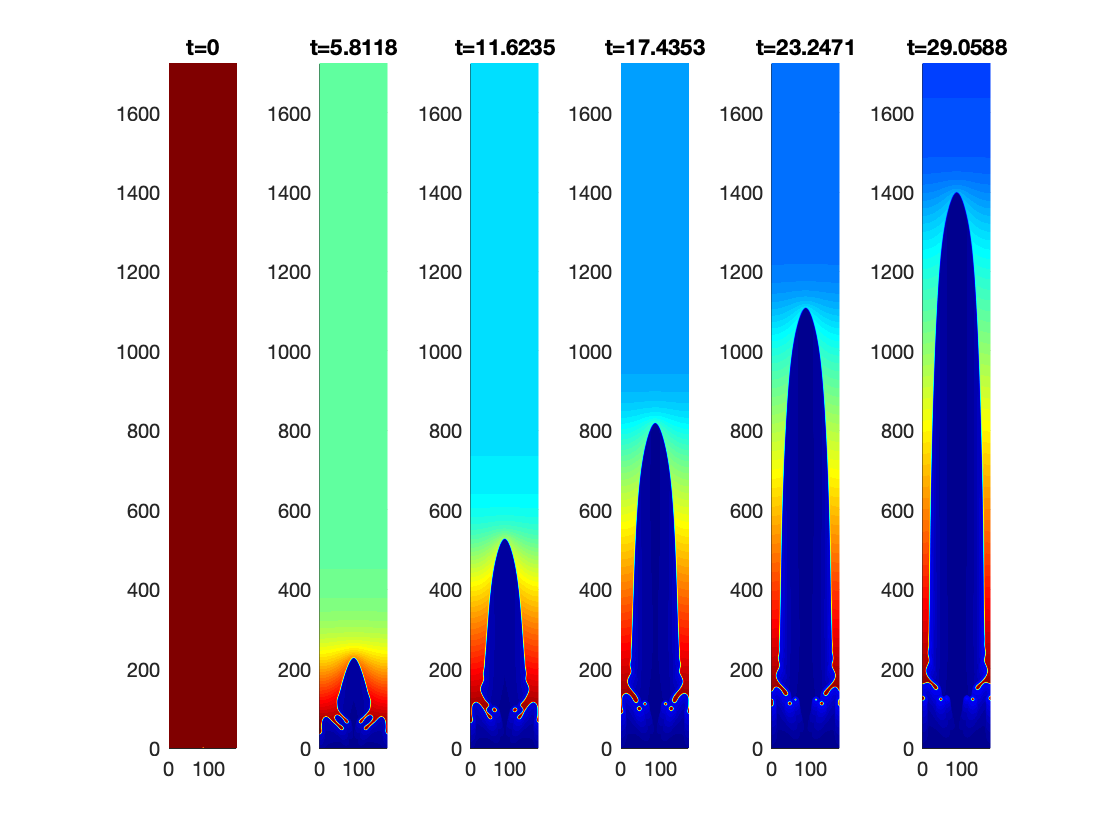
\includegraphics[width=0.7\textwidth]{./figures/cell.png}
     }
     \hfill
     \subfloat[dendrite\label{subfig-2:c/cinf}]{%
       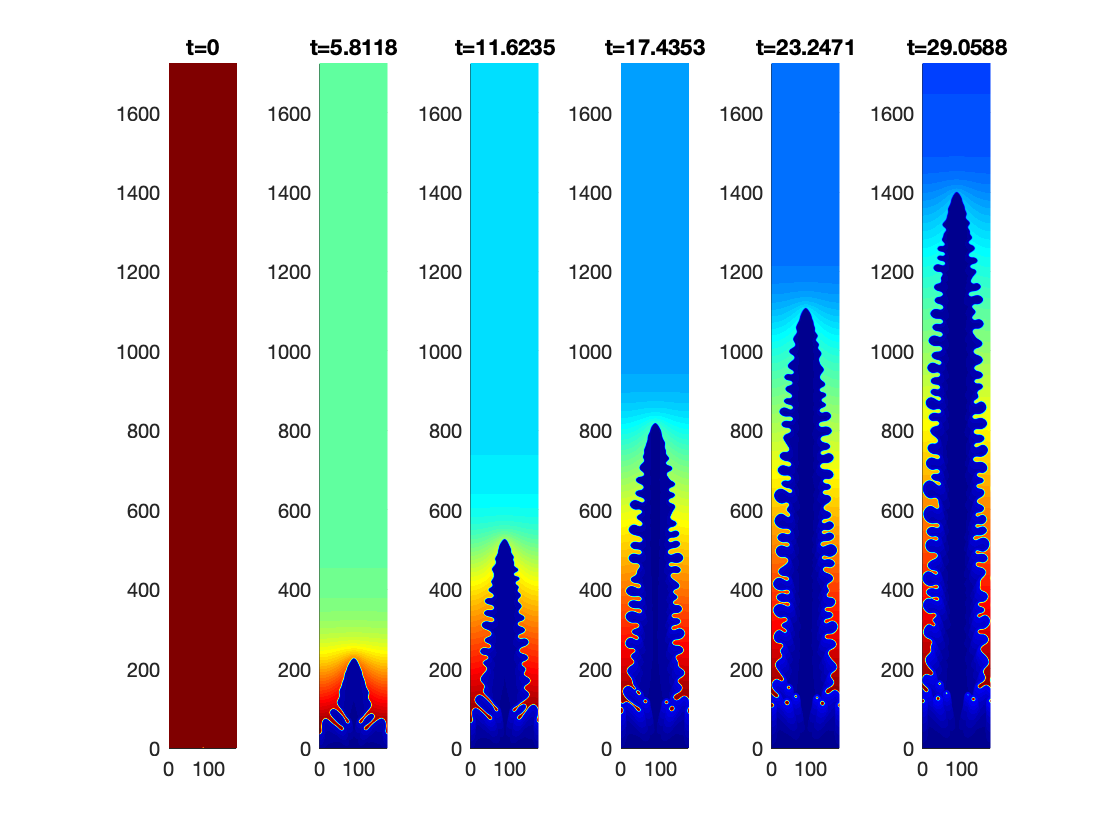
\includegraphics[width=0.7\textwidth]{./figures/dendrite.png}
     }     
     
     \caption{(a) Dendrite morphologies and concentration distributions.(a) $\eta=0$. (b) $\eta=0.05$ Use the same physical parameters of Al-Cu in \cite{Takaki2014}}
     \label{fig:Ech}
   \end{figure}
   




%% \section{}
%% \label{}

%% If you have bibdatabase file and want bibtex to generate the
%% bibitems, please use
%%
\bibliographystyle{unsrt}
\bibliography{Directional-Solidification.bib}



%% else use the following coding to input the bibitems directly in the
%% TeX file.

%\begin{thebibliography}{00}

%% \bibitem{label}
%% Text of bibliographic item


%\end{thebibliography}

\end{document}
\endinput
%%
%% End of file `elsarticle-template-num.tex'.